\documentclass[tikz,border=10pt]{standalone}
\usepackage{tikz}
\usetikzlibrary{positioning, calc, arrows.meta}

\begin{document}
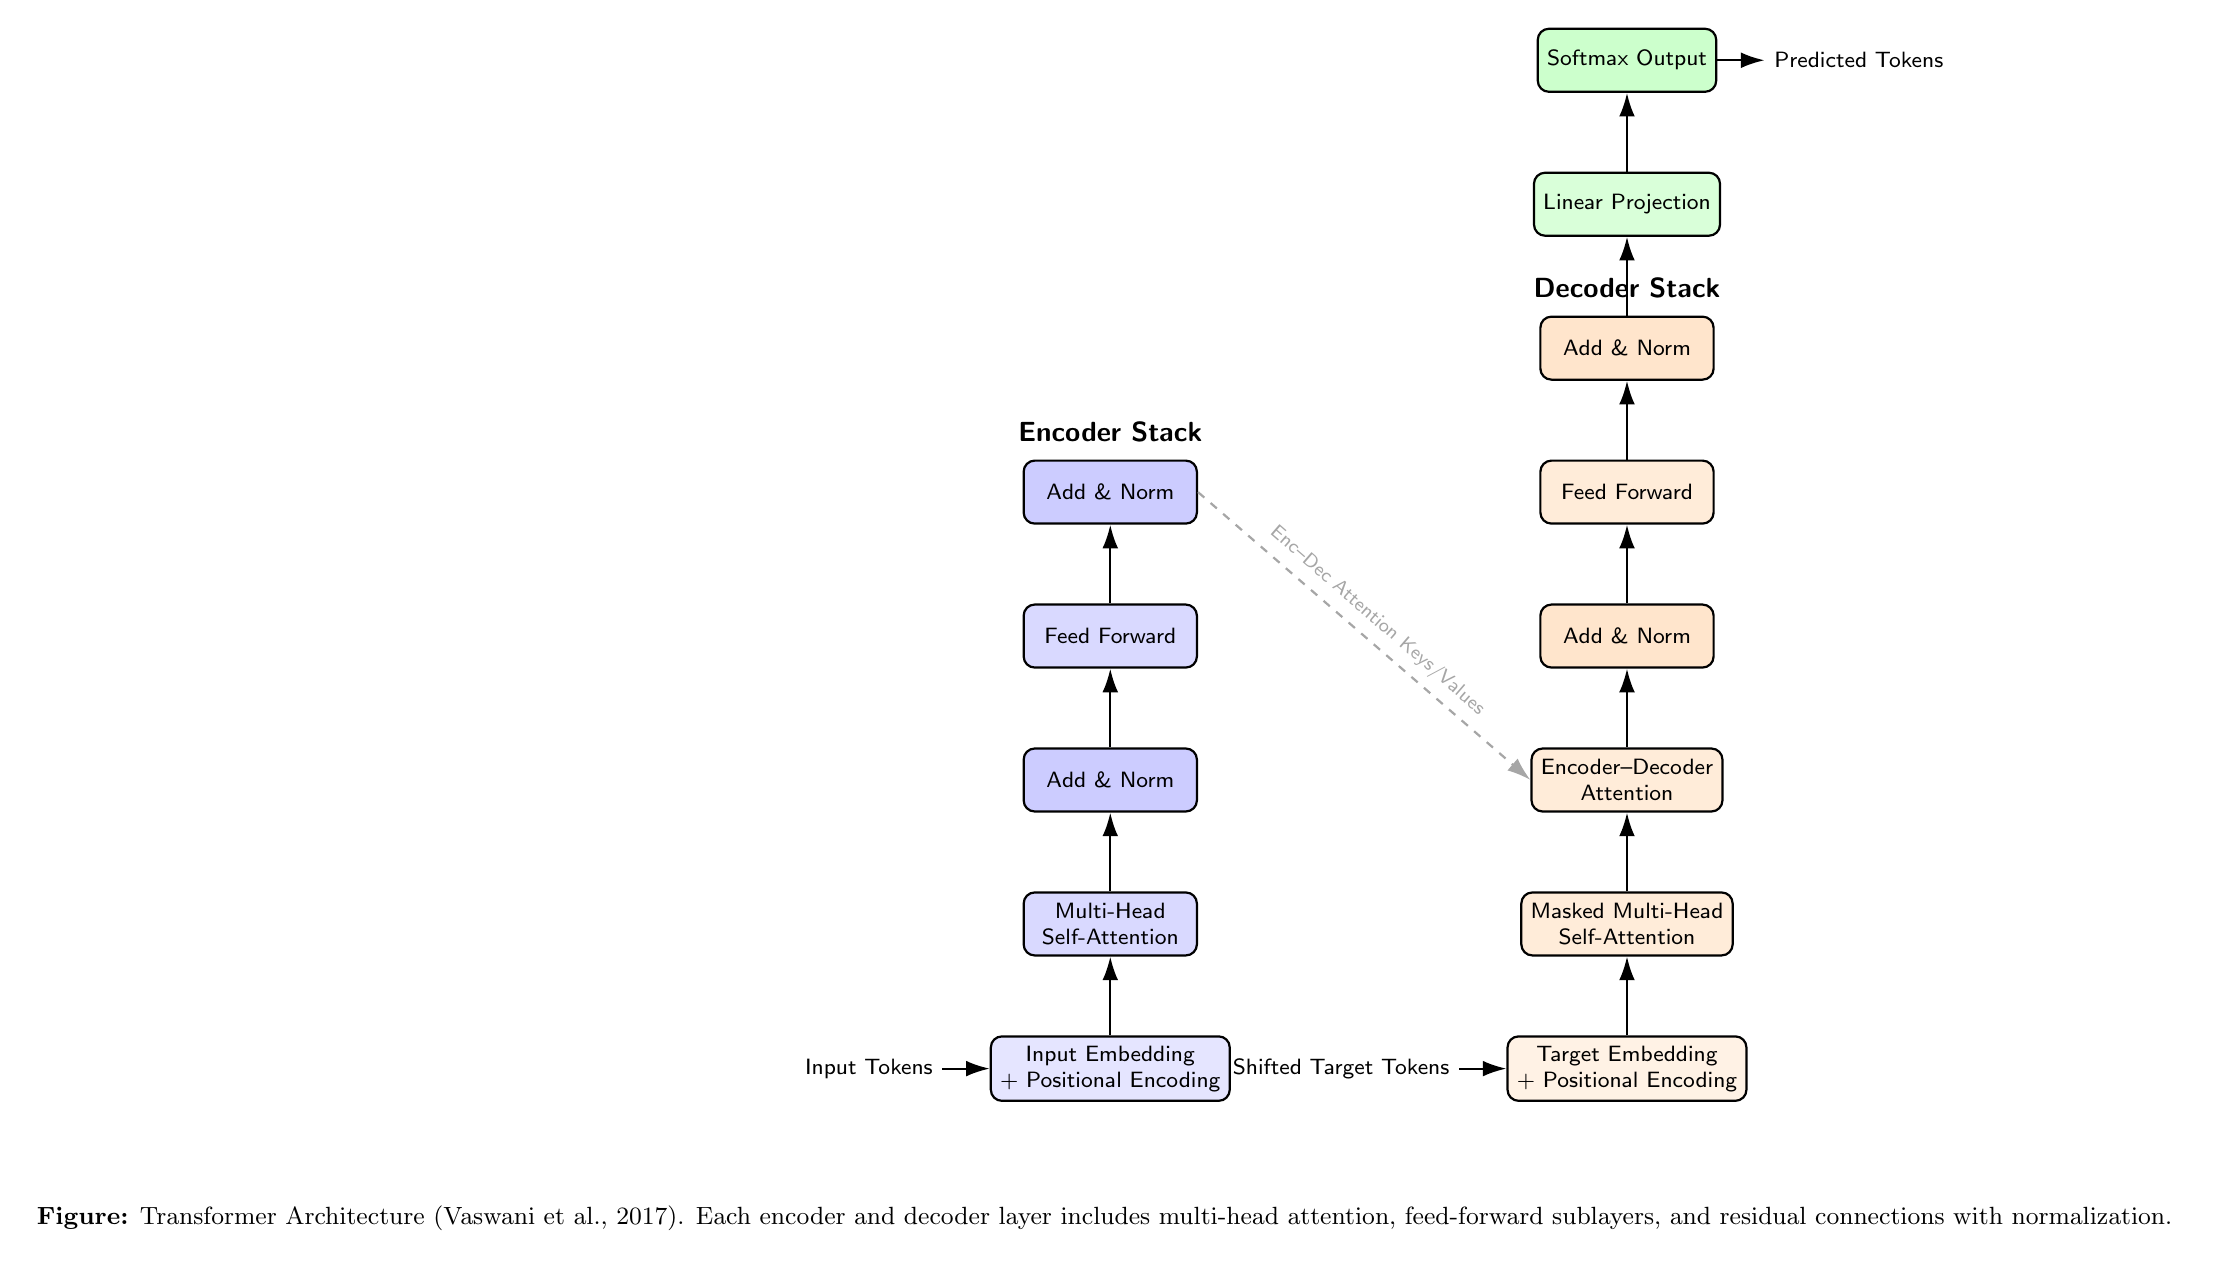
\begin{tikzpicture}[
  font=\sffamily,
  >=Latex,
  layer/.style={rectangle, draw, rounded corners, thick, minimum height=8mm, minimum width=22mm, align=center},
  arrow/.style={-{Latex[length=3mm, width=2mm]}, thick},
  every node/.style={font=\sffamily\footnotesize}
]

%--------------------------------------
% Encoder stack
%--------------------------------------
\node[layer, fill=blue!10] (embed) {Input Embedding\\+ Positional Encoding};
\node[layer, fill=blue!15, above=of embed] (selfattn_enc) {Multi-Head\\Self-Attention};
\node[layer, fill=blue!20, above=of selfattn_enc] (addnorm1_enc) {Add \& Norm};
\node[layer, fill=blue!15, above=of addnorm1_enc] (ffn_enc) {Feed Forward};
\node[layer, fill=blue!20, above=of ffn_enc] (addnorm2_enc) {Add \& Norm};
\node[draw=none, above=0.1cm of addnorm2_enc, font=\sffamily\bfseries] (encoder) {Encoder Stack};

%--------------------------------------
% Decoder stack
%--------------------------------------
\node[layer, fill=orange!10, right=3.5cm of embed] (embed_dec) {Target Embedding\\+ Positional Encoding};
\node[layer, fill=orange!15, above=of embed_dec] (selfattn_dec) {Masked Multi-Head\\Self-Attention};
\node[layer, fill=orange!15, above=of selfattn_dec] (crossattn) {Encoder–Decoder\\Attention};
\node[layer, fill=orange!20, above=of crossattn] (addnorm_dec) {Add \& Norm};
\node[layer, fill=orange!15, above=of addnorm_dec] (ffn_dec) {Feed Forward};
\node[layer, fill=orange!20, above=of ffn_dec] (addnorm2_dec) {Add \& Norm};
\node[draw=none, above=0.1cm of addnorm2_dec, font=\sffamily\bfseries] (decoder) {Decoder Stack};

%--------------------------------------
% Output
%--------------------------------------
\node[layer, fill=green!15, above=1cm of addnorm2_dec] (linear) {Linear Projection};
\node[layer, fill=green!20, above=of linear] (softmax) {Softmax Output};

%--------------------------------------
% Arrows and connections
%--------------------------------------
\draw[arrow] (embed.north) -- (selfattn_enc.south);
\draw[arrow] (selfattn_enc.north) -- (addnorm1_enc.south);
\draw[arrow] (addnorm1_enc.north) -- (ffn_enc.south);
\draw[arrow] (ffn_enc.north) -- (addnorm2_enc.south);

\draw[arrow] (embed_dec.north) -- (selfattn_dec.south);
\draw[arrow] (selfattn_dec.north) -- (crossattn.south);
\draw[arrow] (crossattn.north) -- (addnorm_dec.south);
\draw[arrow] (addnorm_dec.north) -- (ffn_dec.south);
\draw[arrow] (ffn_dec.north) -- (addnorm2_dec.south);
\draw[arrow] (addnorm2_dec.north) -- (linear.south);
\draw[arrow] (linear.north) -- (softmax.south);

% Connection between encoder & decoder
\draw[arrow, dashed, thick, color=gray!70]
  (addnorm2_enc.east) -- node[midway, above, sloped]{\scriptsize Enc–Dec Attention Keys/Values} (crossattn.west);

% Input/output labels
\node[left=0.6cm of embed] (inputtext) {Input Tokens};
\node[left=0.6cm of embed_dec] (targettext) {Shifted Target Tokens};
\node[right=0.6cm of softmax] (outputtext) {Predicted Tokens};

\draw[arrow] (inputtext.east) -- (embed.west);
\draw[arrow] (targettext.east) -- (embed_dec.west);
\draw[arrow] (softmax.east) -- (outputtext.west);

%--------------------------------------
% Caption
%--------------------------------------
\node[below=1.2cm of embed, align=center, font=\small] {
\textbf{Figure:} Transformer Architecture (Vaswani et al., 2017). 
Each encoder and decoder layer includes multi-head attention, 
feed-forward sublayers, and residual connections with normalization.
};

\end{tikzpicture}
\end{document}

